\JWlone{Design}
\label{sec:design}

How did I solve the problem?



%#  BIG PICTURE  ###############################################################
\JWltwo{Big Picture of the Setup}
\label{sec:big-pic}

see figure \ref{fig:overview} and text:

\begin{figure}
  \centering
    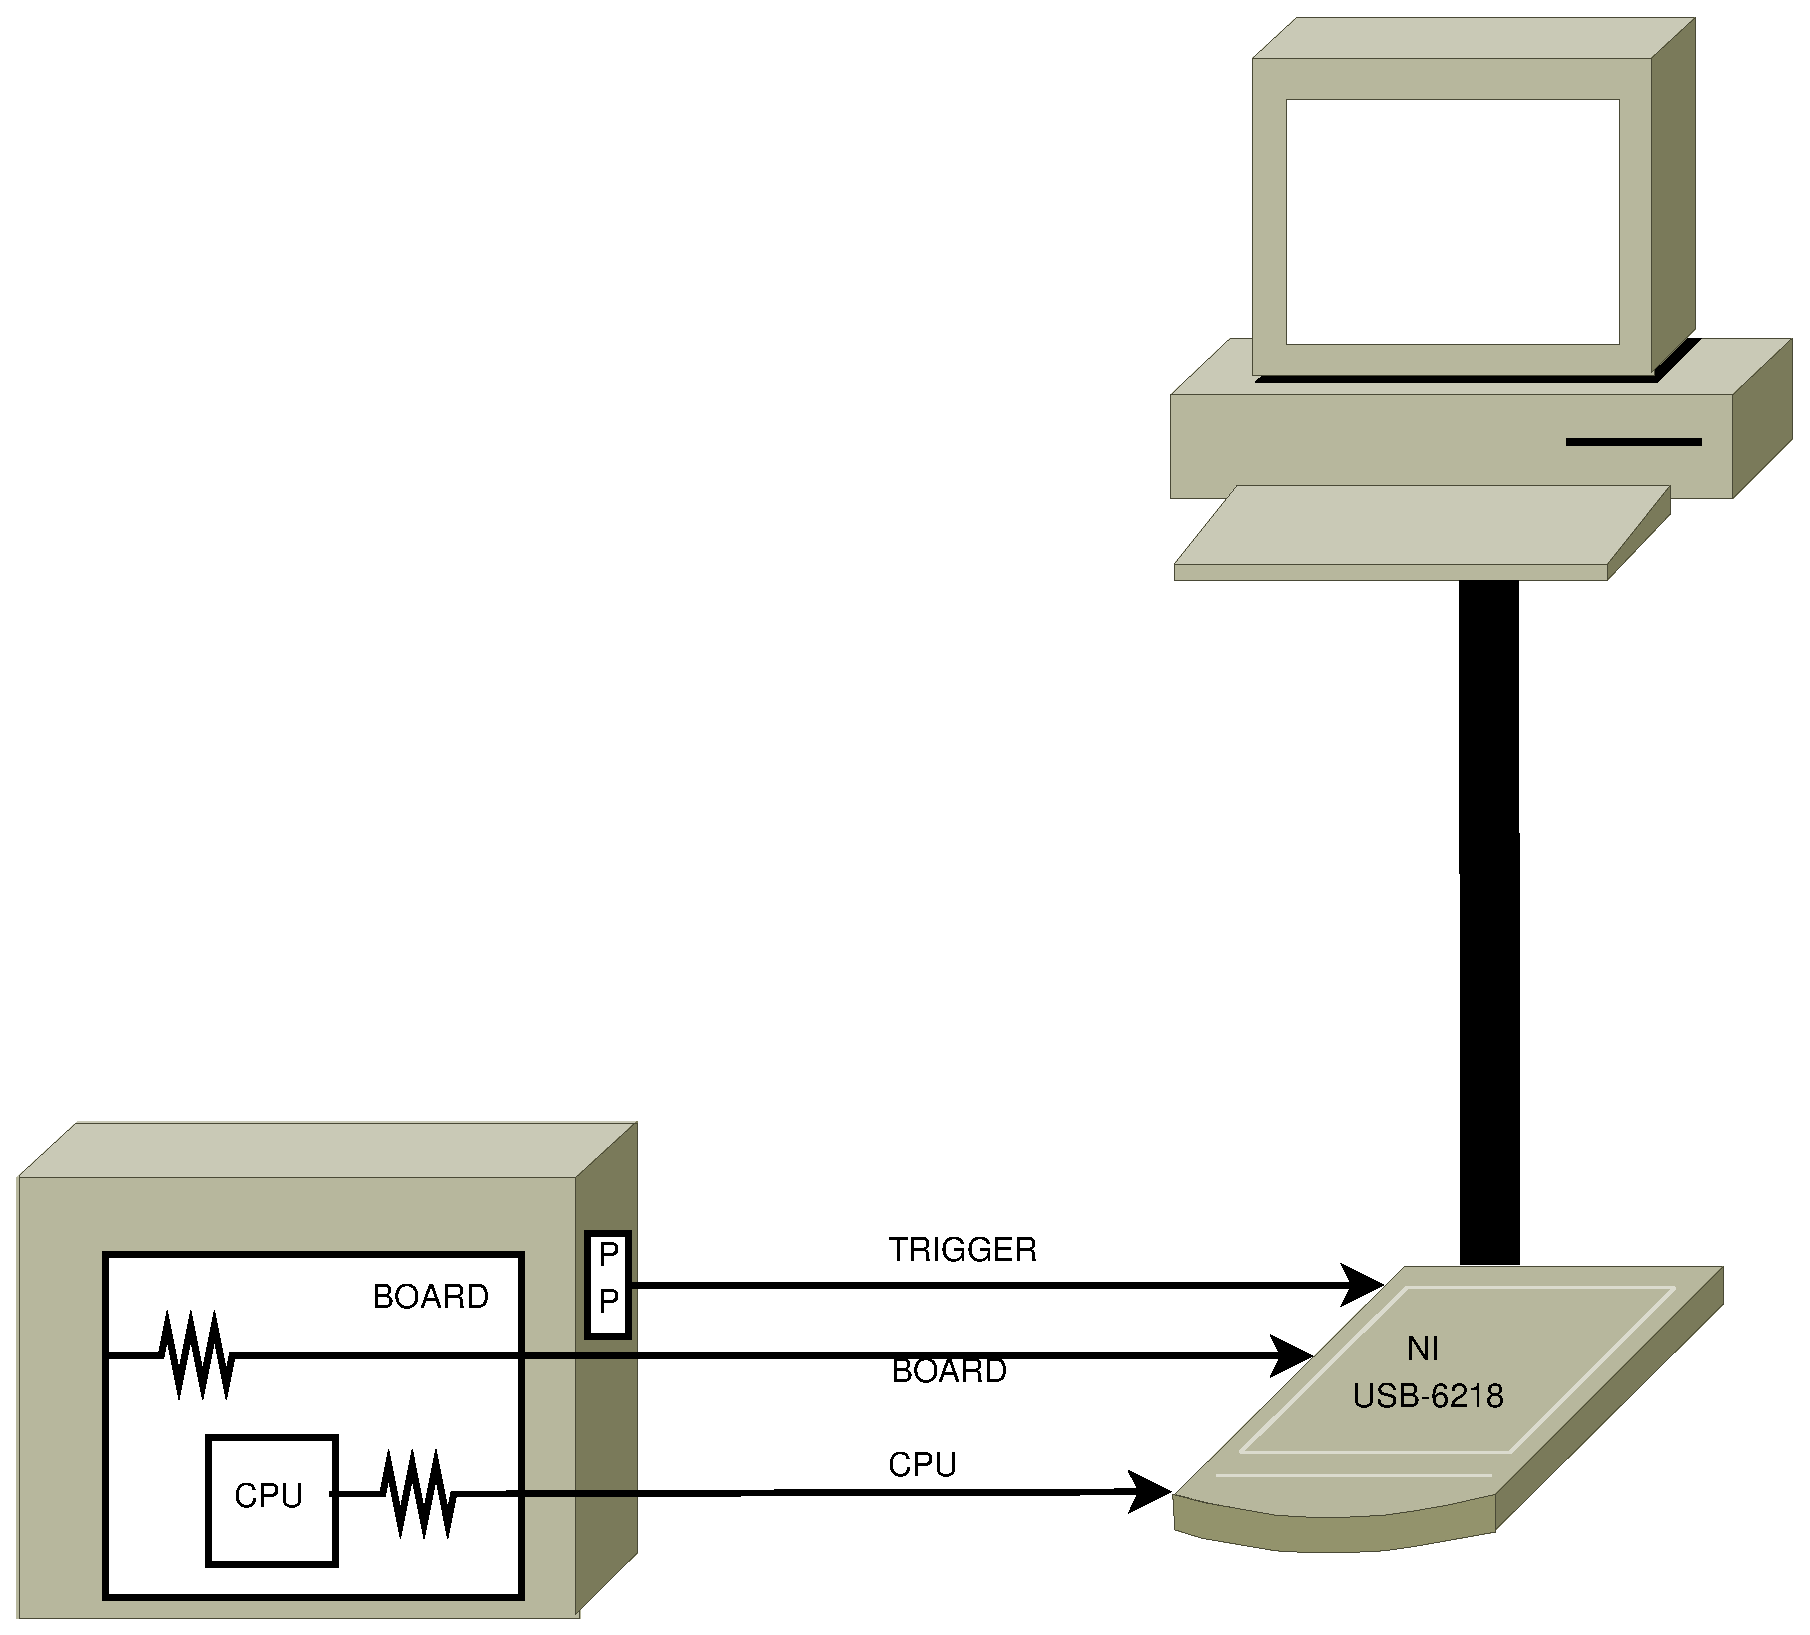
\includegraphics[width=\textwidth]{fig/measuring-overview.eps}
  \caption{Measuring setup overview}
  \label{fig:overview}
\end{figure}

\begin{itemize}

\item Instrumented Sandy Bridge computer counter performance events and is 
      connected to

\item measuring computer which records voltage drops using

\item NI USB-6218.

\end{itemize}

%#  MEASURING SETUP IN DETAIL  #################################################
\JWltwo{Measuring Setup in Detail}
\label{sec:measuring-setup}

In this chapter the measuring setup in detail is presented.


%-  characteristics  -----------------------------------------------------------
\JWlthree{Characteristics}

\begin{itemize}

\item Three differential analog channels: CPU, BOARD, TRIGGER

\item Sampling rate: \SI{50}{\kilo\samples\per\second}

\end{itemize}


%-  wiring scheme  -------------------------------------------------------------
\JWlthree{Wiring Scheme}

In this section a figure of the wiring scheme will be presented. It will contain
every wire, resistor and transistor. It will also include the voltage adjustment
circuit.


%-  measuring device  ----------------------------------------------------------
\JWlthree{Measuring Device}
\label{sec:measuring-device}

For measuring the voltage drops we chose \JWPni from
\JWenterprise{http://www.ni.com}{National Instruments} because it supports high
sampling rates of up to 250000 samples per second
(\SI{250}{\kilo\samples\per\second}) and is very accurate (accuracy $<
\SI{2.69}{\milli\volt}$)\cite{NISpec2009}.


%#  CALCULATION OF THE ELECTRICAL WORK  ########################################
\JWltwo{Calculation of the Eletrical Work}
\label{sec:calc-work}

From elementary physics

\begin{eqnarray}
     U_R & = & R * I \\
  \iff I & = & \frac{U_R}{R}
\end{eqnarray}

and

\begin{equation}
  U_{CPU} + U_{R} = 12 V
\end{equation}

we obtain the instantaneous power of the CPU by measuring the voltage drop
across the (measuring) resistor:

\begin{eqnarray}
P_{CPU}(t) & = & (12V - U_R(t)) * \frac{U_R(t)}{R} \\
           & = & \frac{12V * U_R - {U_R}^2}{R} \\
           & \stackrel{0 < U_R \ll 1}{\approx} & \frac{12V * U_R}{R}.
\end{eqnarray}

Hence, integrating will result in the electrical work

\begin{equation}
  W = \int P_{CPU}(t)dt.
\end{equation}


%#  THE ENERGY MODEL  ##########################################################
\JWltwo{The Energy Model}
\label{sec:model}

In this section the mathematical and formal methods to find a good subset of
events and their coefficients is presented.

%-  the model's properties  ----------------------------------------------------
\JWltwo{The Model's Properties}
\label{sec:model-properties}

In this work, an energy model is considered as a linear formula. A system with
$N$ CPUs/cores which is able to monitor $M$ performance events per core
simultaneously is described here. Additionally to the per-core event counters,
$K$ system-wide event counters make the model up. In the formal description (see
section \ref{sec:model-pratical} for the practical implementation) we assume
four functions providing the actual values:

\begin{itemize}

\item $g(k)$ the global event $k$'s count in the observed period of time

\item $c(n, m)$ the performance event $m$'s count in the observed period of time
      on CPU/core $n$

\item $w_g(k)$ the global event $k$'s weight in \si{\joule}

\item $w_c(n, m)$ the weight of performance event $m$ in \si{\joule} on core
$n$

\end{itemize}

Though, a energy model equates to

\begin{equation}
W = \sum\limits_{k=0}^K g(m) w_g(m) +
\sum\limits_{n=0}^N \sum\limits_{m=0}^M c(n, m) w_c(n,m)
\end{equation}

. The functions $g$ and $c$ contain the system's life data whereas $w_g$ and
$w_c$ can be calculated a priori as done in this work. Obviously the selection
of the events and their respective weights highly depend on the type of
microprocessor.


%-  minimizing the counter set  ------------------------------------------------
\JWlthree{Minimizing the Set of Performance Events}
\label{sec:min-events}

After having seen (section \ref{sec:model-properties}) what exactly makes up a
model, it crucial to find a small and powerful set of performance events we
actually use. It's not practical to take into account all the events the
microprocessor is aware of. Today's processors offer a lot more events then they
have counters to count them at once \cite{intel2011softdev1}.

The approach to find a reasonable subset of $N$ events (of $A$ available) used
in this work can be summed up to:

\begin{itemize}

\item Choose $p$ test programs which utilize the CPU differently. The test
programs have to be independent from external events. We consider subsequent
runs of the test programs as equal.

\item Divide the $A$ available events in $g$ disjoint, non-empty sets $E_{1..g}$
of size up to $N$

\item For each set $E_{1..g}$, run all the $p$ test programs and record the
electrical work and the event counters of the set's events

\item The electrical work of each of the runs of a test program should be
roughly equal.

\item Folding all the results, we gain a vector $W_{1..p}$ of the electrical
work a run of each of the test programs consumes. Additionally, we gain a matrix
$C = [c_{1..p,1..N}]$ containing each event counter's value for a run of each of
the test programs.

\end{itemize}

provide because we need to count them simultaneously. 

\begin{itemize}

\item Take all counters,

\item eliminate equal counters,

\item eliminate linear dependent counters,

\item generate the 5 best models of sizes 1..size(counters),

\item eliminate all counters which appear in no model.

\item Perform exhaustive search on the still-living counters.

\end{itemize}


% vim: set spell spelllang=en_us fileencoding=utf8 :
